\section{异常类\texttt{std::exception}相关}
\lstinline@std::exception@ 定义于头文件 \lstinline@exception@ 当中,它的成员函数除了默认构造函数、拷贝构造函数、析构函数和赋值运算符之外,就只有一个虚函数 \lstinline@what()@。单纯的 \lstinline@std::exception@ 对象的意义不大,但它的常量引用,也就是 \lstinline@const std::exception&@ 类型,这个类型是很有用的。\par
我们曾说过,在异常对象的类型匹配过程中,基类的常量引用可以接收派生类的对象——所以,我们可以抛出它的派生类对象,并用基类引用来接收。这样一来,无论我们抛出的是哪个派生类对象,\lstinline@const std::exception&@ 都可以接收它,而不会遗漏(如果一个 \lstinline@throw@ 找不到能够捕获它的 \lstinline@catch@,将会导致程序终止,我们已经提过了)。\par
图12.1展示了 \lstinline@std::exception@ 的各个派生类,它们定义在不同的头文件中。\par
\begin{figure}[htbp]
    \centering
    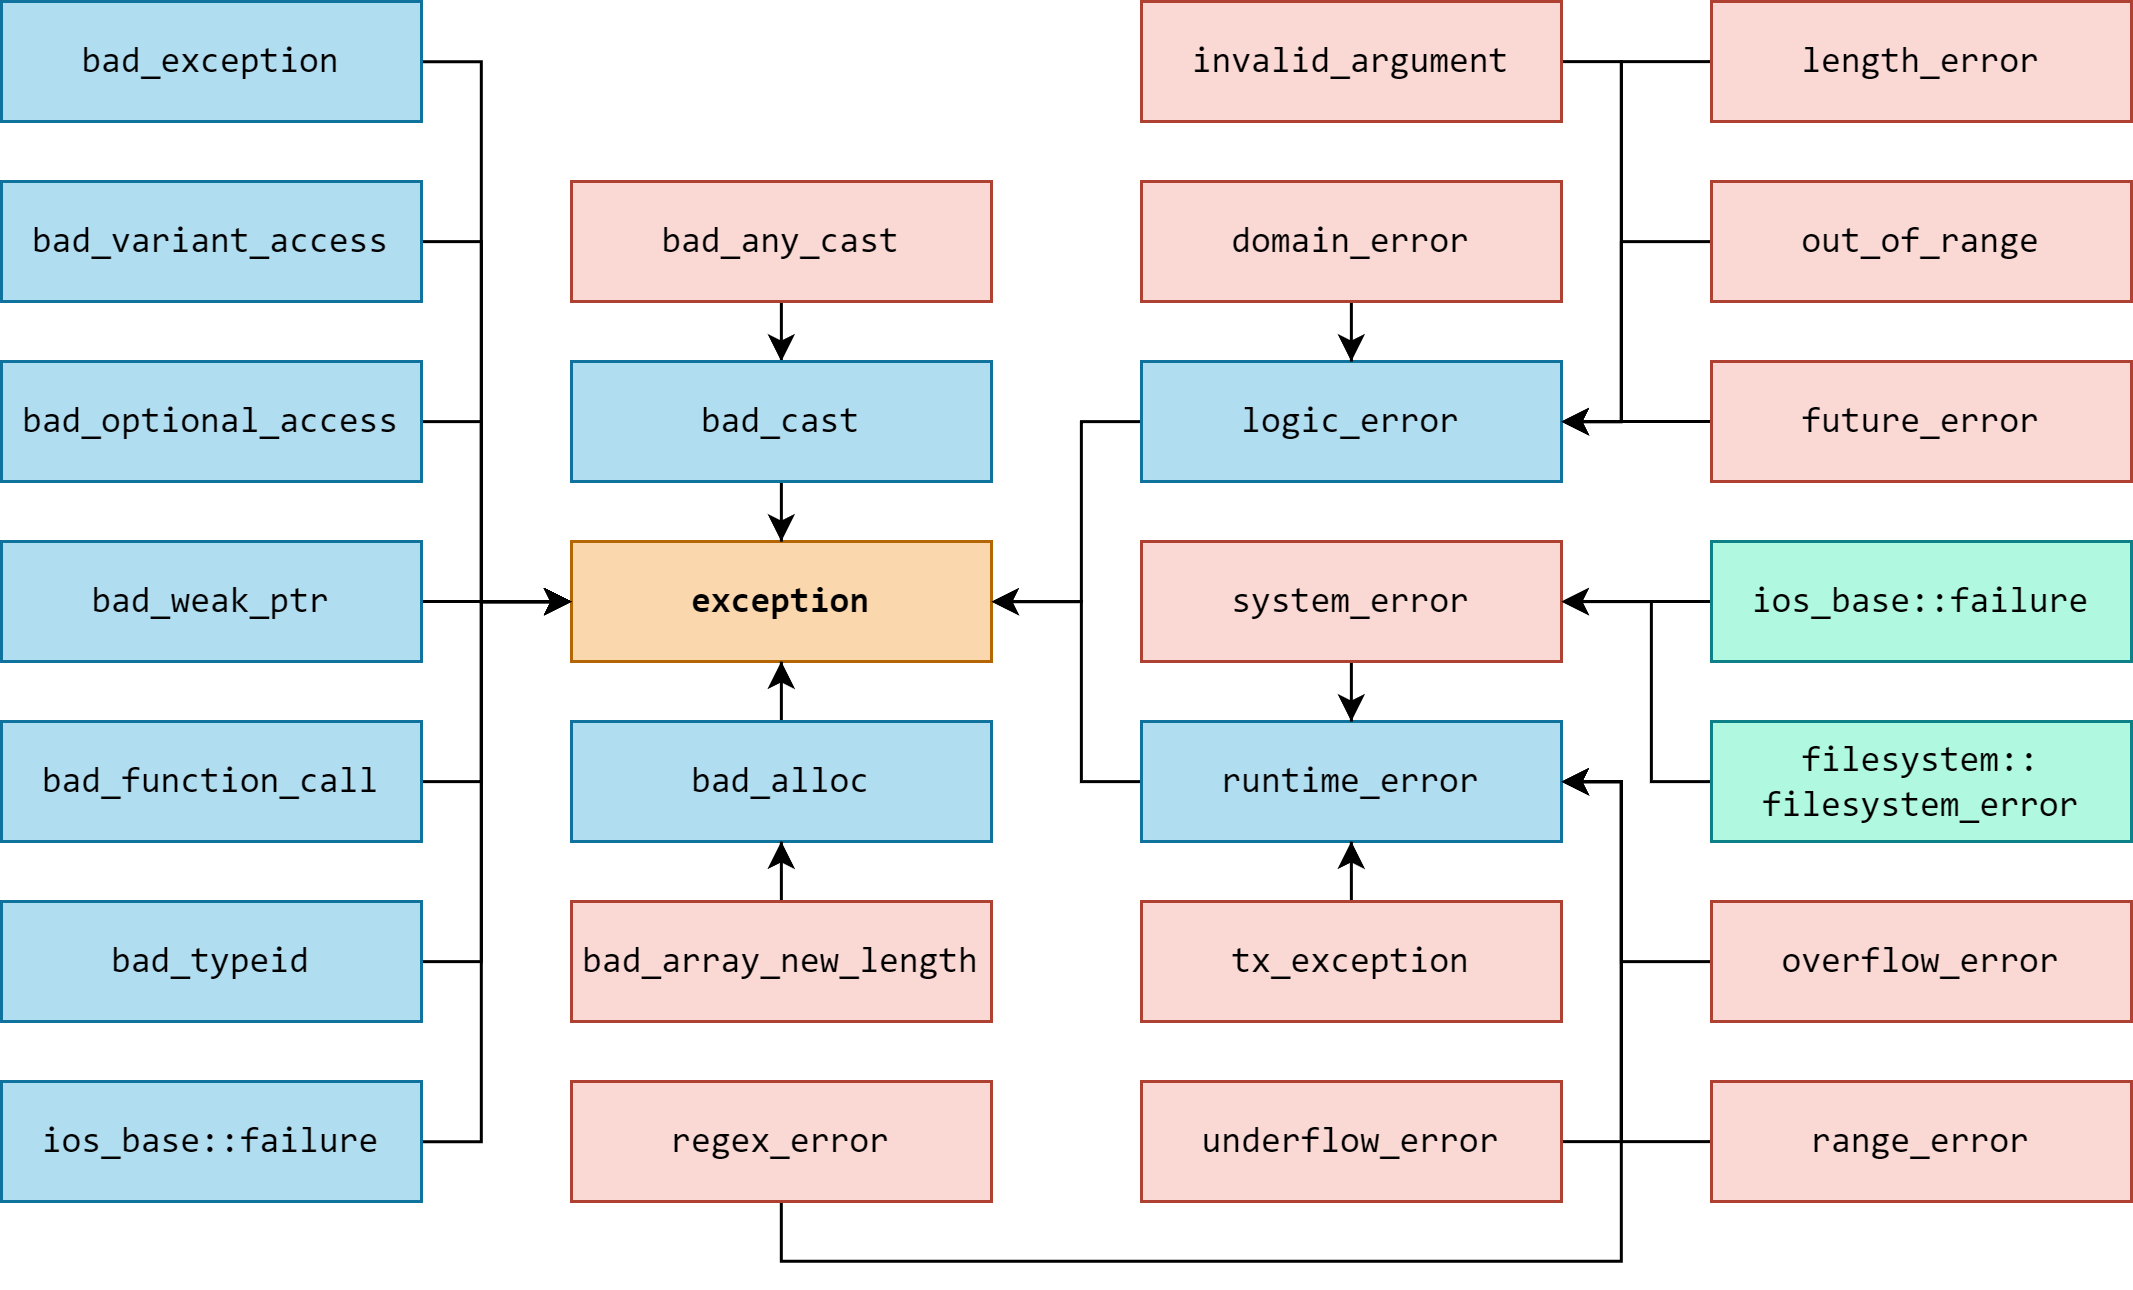
\includegraphics[width=\textwidth]{../images/generalized_parts/12_std_exception_family.drawio.png}
    \caption{\lstinline@std::exception@ 家族(C++17标准)}
    \footnotesize{默认在 \lstinline@std@ 命名空间下;颜色仅用以区分继承的层级}
\end{figure}
举个例子,\lstinline@std::bad_alloc@ 表示动态内存分配失败。导致这个问题出现的可能原因是内存泄漏导致堆空间不足以继续分配,我们就不去细研究它了。以下代码可以演示这样的例子:
\begin{lstlisting}
//记得#include<exception>
    try {
        while (true)
            new int[100000ul]; //不停地进行内存泄漏操作
    } catch (const std::exception &msg) { //用std::exception常量引用接收参数
        std::cout << "An exception has been caught:\n" << msg.what();
    }
\end{lstlisting}
这段代码的运行结果如下:\\\noindent\rule{\linewidth}{.2pt}\texttt{
{\kaishu\color{gray}(开始运行一段时间后)}\\
An exception has been caught:\\
std::bad\_alloc
}\\\noindent\rule{\linewidth}{.2pt}\par
\lstinline@what@ 是虚函数,所以只要 \lstinline@msg@ 是对 \lstinline@std::bac_alloc@ 对象的引用,那么它调用的 \lstinline@what@ 就是后者的成员函数。这是一种多态。\par
\lstinline@what@ 的返回值是 \lstinline@const char*@ 字符串,代表的就是这个异常的种类。对于 \lstinline@std::bad_alloc@ 来说,它的返回值就是我们在运行结果当中看到的那样。
再来看看 \lstinline@std::out_of_range@ 的例子,我们可以用 \lstinline@std::vector@ 对象的元素访问来触发它。
\begin{lstlisting}
    std::vector<int> vec {1,2,3,4,5};
    try {
        std::cout << vec.at(5); //试图访问5号元素,但正确的范围是0~4
    } catch (const std::exception &msg) {
        std::cout << "An exception has been caught:\n" << msg.what();
    }
\end{lstlisting}
这段代码的运行结果是:\\\noindent\rule{\linewidth}{.2pt}\texttt{
An exception has been caught:\\
vector::\_M\_range\_check: \_\_n (which is 5) >= this->size() (which is 5)
}\\\noindent\rule{\linewidth}{.2pt}\par
这里的 \lstinline@what@ 返回内容清楚明白,意思就是提供的参数 \lstinline@n@ 大于等于 \lstinline@this->size()@,这就是范围错误了。\par
顺便一提,\lstinline@std::out_of_range@ 继承自 \lstinline@std::logic_error@,它们都定义在 \lstinline@stdexcept@ 库中。但是我们即便不包含这个库也能用,这是因为 \lstinline@vector@ 库中已经包含过它了。\par
\subsection*{实操:为 \texttt{user::array::at}设计异常抛出}
接下来我们来尝试修改一下曾经写过的 \lstinline@std::array@ 的 \lstinline@at@ 函数,当下标范围不合理时,让它抛出 \lstinline@std::out_of_range@ 对象。\pagebreak
\begin{lstlisting}
//记得#include<stdexcept>和#include<string>
template<typename T, std::size_t N>
constexpr T& user::array<T, N>::at(std::size_t pos) {
    if (pos >= N) { //范围错误,应当抛出异常
        std::string msg {}; //用std::string对象拼接内容效率更高
        msg += "array::_M_range_check: __n (which is ";
        msg += std::to_string(pos); //std::to_string可以把数字变成string对象
        msg += ") >= this->size() (which is ";
        (msg += std::to_string(N)) += ")"; //至此,拼接完成
        throw std::out_of_range(msg); //out_of_range有面向string的构造函数
    }
    return _elem[pos];
}
\end{lstlisting}
常成员函数的版本同上,不再赘述了,我们只来讲一讲这里涉及到的细节就好。\par
首先,我们在这里选择使用 \lstinline@std::string@ 来构造 \lstinline@std::out_of_range@,这是出于两点原因:其一,是后者本来就有这样构造函数 \lstinline@out_of_range(const std::string&)@,我们可以很方便地构造对象来返回;其二,是 \lstinline@std::string@ 所重载的 \lstinline@+=@ 运算符十分方便进行内容拼接,我们不用写一个 \lstinline@char[]@ 数组然后反复用 \lstinline@std::strcpy@ 来向其中添加内容。\par
这里我们还用到了 \lstinline@string@ 库中的函数 \lstinline@std::to_string@。它对常见的整数和浮点数类型都有重载,我们可以通过这个函数把整数/浮点数变成内容相同的 \lstinline@std::string@ 对象。这样我们也就不需要自己写一个数字到字符的转换函数了,是不是很方便?\par
\subsection*{\texttt{noexcept}简介}
在C++中,我们可以按照抛出异常的情况,把函数分为两类:\textbf{不会抛出异常的函数}和\textbf{可能会抛出异常的函数}。默认情况下,所有的函数都是后者——可能会抛出异常的函数。\par
既然默认任何一个函数都是可能会抛出异常的,那么编译器就必须为每一个函数产生额外的代码,用以正确地处理栈回溯(别看我们写一个 \lstinline@throw@ 那么轻巧,实际上编译器要为此做很多工作的)。但是有些时候,我们写的函数很简单,压根不需要抛出什么异常。这个时候,我们就可以把它声明为``不会抛出异常的函数''。这样一来,编译器就不会为它生成多余的代码,这样能提高程序的效率——毕竟,C++是一种注重执行效率的语言。\par
声明一个不会抛出异常的函数,需要使用 \lstinline@noexcept@ 说明符。
\begin{lstlisting}
unsigned factorial(unsigned)noexcept; //声明,这个函数不会抛出异常
unsigned factorial(unsigned n)noexcept { //定义,这个函数不会抛出异常
    if (n == 0)
        return 1;
    return n * factorial(n - 1); //的确,这里没有抛出异常的需求和可能性
}
\end{lstlisting}\par
注意 \lstinline@noexcept@ 本身是函数的一部分,无论声明还是定义都必须带上它。\par
有了 \lstinline@noexcept@ 之后,编译器就放心地把异常处理有关的代码省略掉了;但是请注意,这并不意味着编译器对我们的函数进行了语法检查——它只是听信了你的一面之词而已!倘若你真的在这个函数中抛出了异常——或者做得更隐蔽一点,在这个调用了一个``可能会抛出异常的函数'',编译器也是不会管你的\footnote{有些编译器倒是可以提出警告或者给出报错,但其作用范围也很有限。}。\par
如果真的发生了这种事情,会怎么样呢?比如说,栈回溯没有正常发生,因为你当初信誓旦旦说这个函数不会抛出异常,编译器就把这段代码优化掉了。所以说我们在写代码的时候还是要注意一点,如果一个函数是 \lstinline@noexcept@ 的,那么它本身不应该抛出异常;它调用的那些函数和运算符,都应该是 \lstinline@noexcept@ 的——退一步讲,不能抛出异常的。只有这样,我们才能保证这个程序本身既安全,又高效。\par
不过你可能会想:标准库里那么多函数,我怎么知道哪一个是 \lstinline@noexcept@ 哪一个不是啊?这个时候我们有两种办法:一是查文档或者源代码,标注了 \lstinline@noexcept@ 的是不会抛出异常的,否则就是可能抛出异常的;二是可以用 \lstinline@noexcept@ 运算符来取定某个表达式,观察它的返回值。
\begin{lstlisting}
void func()noexcept { }
void func(int n) { }
int main() {
    std::cout << noexcept(func()) << std::endl; //1
    std::cout << noexcept(func(1)); //0
    std::vector<int> vec(3); //vec的长度为3
    std::cout << noexcept(vec.at(3)) << std::endl; //0
    std::cout << noexcept(vec.at(2)) << std::endl; //仍然是0
\end{lstlisting}
读者会发现 \lstinline@noexcept(vec.at(2))@ 的返回值依然是 \lstinline@0@,这说明 \lstinline@noexcept@ 的返回值其实是与表达式中的具体参数无关的。\par
